\usetikzlibrary{patterns,calc,decorations.pathreplacing}

\pgfdeclarehorizontalshading{randomgray}{100bp}{
color(0bp)=(gray!10);
color(100bp)=(gray!90)
}

\begin{tikzpicture}

  % Define the dimensions of the rectangles
  \def\cornerradius{3pt}
  \def\rectWidth{1.5cm}
  \def\rectHeight{3.5cm}
  \def\spacing{0.34cm}
  \def\rightRectSpacing{0.8cm} % Spacing between right rectangles
  \def\encoderLabelSpacing{0.17cm} % Spacing between encoders and labels

  % Define the colors
  \definecolor{encoder_color}{HTML}{96B24D}
  \definecolor{thiscolor}{HTML}{0078AD} 
  \definecolor{random_color}{HTML}{00B5FF}
  \definecolor{st_color}{HTML}{FF4A00} 
        
    % Draw category labels FIRST (so they are in the back)
    \begin{scope}[xshift=-2.16cm, yshift=-0.4cm]
        \node[fill=gray!10, draw=none, minimum width=2.5cm, minimum height=7.75cm, anchor=center, rounded corners=\cornerradius] 
            (background) at (0, -0.42) {};
        \draw[black, very thick, rounded corners=\cornerradius] 
            ($(background.north west)$) rectangle ($(background.south east)$);

        \node[align=center, font=\footnotesize\sffamily, text=black] at (0, 1.01*\rectHeight - \spacing) {\textbf{Pretraining Data}}; 
        
        \foreach \y/\label in {
          1/Space-Time,
          2/S1-SAR,
          3/S2-RGB,
          4/S2-SWIR,
          5/S2-Red-Edge,
          6/S2-NIR-10m,
          7/S2-NIR-20m,
          8/S2-NDVI,
          9/Space,
          10/Elevation, 
          11/Dynamic World,
          12/World Cereal,
          13/Time,
          14/Weather,
          15/TerraClimate, 
          16/Nightlights,
          17/Static,
          18/Population,
          19/Location, 
          20/Dynamic World,
          21/World Cereal
        } {
          % Conditional for black background
          \ifthenelse{
            \equal{\label}{Space-Time} \OR \equal{\label}{Time} \OR 
            \equal{\label}{Space} \OR \equal{\label}{Static}
          }{
            \node[align=center, font=\footnotesize, fill=black, text=white, 
                  rounded corners=2pt, inner sep=1pt] (cg\y) at (0, \rectHeight-\y*\spacing - \spacing) {\textbf{\label}}; 
          }{
            \node[align=center, font=\footnotesize] (cg\y) at (0, \rectHeight-\y*\spacing - \spacing) {\label}; 
          }
        }
    
    \end{scope}
  
  % Online encoder LEFT
  \node[inner sep=0, anchor=north west] at (-2.1*\rectHeight, 0.7*\rectHeight) {
    \begin{tikzpicture}
        
      \fill[gray!10, rounded corners=\cornerradius] (0, -0.04*\rectWidth) rectangle (\rectWidth, 0.51*\rectHeight + -0.04*\rectWidth);
      \draw[black, very thick, rounded corners=\cornerradius] (0, -0.04*\rectWidth) rectangle (\rectWidth, 0.51*\rectHeight + -0.04*\rectWidth ); 

     \def\COLORS_LIST{{"pink", "pink", "yellow", "yellow", "yellow"}}
     \def\FILES_LIST{{"srtm2.png", "srtm.png", "rgb3.png", "rgb2.png", "rgb1.png"}}

      \foreach \i in {1,...,5} {
        % Get the filename from the list
        \pgfmathparse{\FILES_LIST[\i-1]}
        \edef\imagename{\pgfmathresult}
    
        % Resolve file path dynamically
        \edef\imagepath{pics/\imagename} 
        \pgfmathsetlengthmacro{\tileWidth}{0.2*\rectWidth}
    
        % Place the image as a tile
        \node at (1.29*\rectWidth, -0.035*\rectWidth + 0.1*\rectHeight*\i) {
            \includegraphics[width=\tileWidth]{\imagepath}
        };

        \pgfmathparse{\COLORS_LIST[\i-1]} % \i starts from 1, array index starts from 0
        \edef\THIS_COLOR{\pgfmathresult} 
        
        \fill[color=\THIS_COLOR] (1.25*\rectWidth, -0.04*\rectWidth + 0.1*\rectHeight*\i) 
          rectangle (1.05*\rectWidth, -0.04*\rectWidth + 0.1*\rectHeight*\i - 0.2*\rectWidth);
        \node[font=\footnotesize, align=center] at (1.09*\rectWidth, -0.09*\rectWidth + 0.1*\rectHeight*\i) {$\mathtt{e}$};
      }
      
      \foreach \i in {1,...,5} {
        % Apply the custom gradient shading
        \shade[shading=randomgray] 
            (-0.25*\rectWidth, -0.04*\rectWidth + 0.1*\rectHeight*\i) 
            rectangle (-0.05*\rectWidth, -0.04*\rectWidth + 0.1*\rectHeight*\i - 0.2*\rectWidth);
      }
      
      \draw[-, thick] (-0.3*\rectWidth, -0.04*\rectWidth + 0.5*\rectHeight) -- (-0.3*\rectWidth, -0.01*\rectWidth);
      \draw[->, thick] (-0.3*\rectWidth, -0.02*\rectWidth + 0.25*\rectHeight) -- (-0.5*\rectWidth, -0.02*\rectWidth + 0.25*\rectHeight);
      \draw[-, thick] (1.55*\rectWidth, -0.04*\rectWidth + 0.5*\rectHeight) -- (1.55*\rectWidth, -0.01*\rectWidth);

      % \draw[->, thick, dashed, dash pattern=on 2pt off 1pt] (0.5*\rectWidth, -0.04*\rectWidth) -- (0.5*\rectWidth, -0.71*\rightRectSpacing);
      % \node[font=\scriptsize, align=center] at (0.53*\rectWidth, -0.28*\rightRectSpacing) {EMA};
      \node[font=\footnotesize, align=center] at (0.15*\rectWidth, 0.335*\rectHeight) {Online\\Encoder};
      \node[font=\footnotesize, align=center] at (0.44*\rectWidth, 0.12*\rectHeight) {$\theta$};
      \node[circle, draw=black, fill=black, text=white, font=\bfseries, minimum size=0.1cm, align=center] at (0.44*\rectWidth, 0.44*\rectHeight) {2};
    \end{tikzpicture}
  };


  \node[circle, draw=black, fill=black, text=white, font=\bfseries, inner sep=0.2pt, align=center] at (-3.82, 0.4) {1};
  \node[circle, draw=black, fill=black, text=white, font=\bfseries, inner sep=0.2pt, align=center] at (-0.5, 0.4) {1};
        
  \node[font=\footnotesize] at (-7.2, 2.7) {Global pretraining task};
  \node[font=\footnotesize] at (2.9, 2.7) {Local pretraining task};
  
  \draw[->, thick] (-0.6*\rectWidth, -0.375*\rectHeight) -- (0.34*\rectWidth, -0.375*\rectHeight);
  \draw[->, thick] (-0.6*\rectWidth, 0.44*\rectHeight) -- (-0.06*\rectWidth, 0.44*\rectHeight);
  \draw[->, thick] (-2.28*\rectWidth, -0.625*\rectHeight) -- (-2.82*\rectWidth, -0.625*\rectHeight);
  \draw[->, thick] (-2.28*\rectWidth, 0.44*\rectHeight) -- (-2.82*\rectWidth, 0.44*\rectHeight);

  % bottom left legend
  \node at (-8.7, -3.6) {
    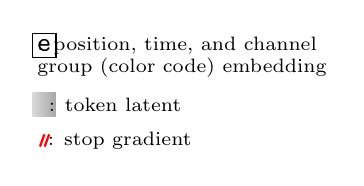
\begin{tikzpicture}          
      \draw[black] (0.1*\rectWidth, 0.1*\rectWidth) 
          rectangle (-0.1*\rectWidth, -0.1*\rectWidth);
      \node[align=center] at (0, 0) {$\mathtt{e}$};
      \node[font=\scriptsize, align=left] at (1.75, -0.15) { : position, time, and channel \\ group (color code) embedding};
      
      \shade[shading=randomgray] (0.1*\rectWidth, 0.1*\rectWidth - 0.5*\rectWidth) 
          rectangle (-0.1*\rectWidth, -0.1*\rectWidth - 0.5*\rectWidth);
      \node[font=\scriptsize, align=left] at (0.9, -0.15 - 0.5*\rectWidth) { : token latent};
      
      % Add the red lines for stop gradient in separate scopes
      \begin{scope}[rotate around={-20:(-0.02*\rectWidth, -0.815*\rectWidth)}]
          \draw[red, thick] (-0.02*\rectWidth, -0.86*\rectWidth) -- (-0.02*\rectWidth, -0.75*\rectWidth);
      \end{scope}
      \begin{scope}[rotate around={-20:(0.02*\rectWidth, -0.815*\rectWidth)}]
          \draw[red, thick] (0.02*\rectWidth, -0.86*\rectWidth) -- (0.02*\rectWidth, -0.75*\rectWidth);
      \end{scope}
      \node[font=\scriptsize, align=left] at (0.96, -0.15 - 0.8*\rectWidth) { : stop gradient};
    \end{tikzpicture}
  };

  % bottom right legend
  \node at (2.8, -3.8) {
    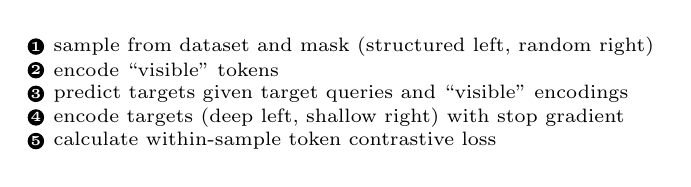
\begin{tikzpicture}
      \node[circle, draw=black, fill=black, text=white, font=\bfseries, inner sep=0.2pt, align=center] at (-0.1, 0) {\tiny{1}};
      \node[font=\scriptsize, anchor=west] at (0, 0) {sample from dataset and mask (structured left, random right)};

      \node[circle, draw=black, fill=black, text=white, font=\bfseries, inner sep=0.2pt, align=center] at (-0.1, -0.3) {\tiny{2}};
      \node[font=\scriptsize, anchor=west] at (0, -0.3) {encode ``visible'' tokens};

      \node[circle, draw=black, fill=black, text=white, font=\bfseries, inner sep=0.2pt, align=center] at (-0.1, -0.6) {\tiny{3}};
      \node[font=\scriptsize, anchor=west] at (0, -0.6) {predict targets given target queries and ``visible'' encodings};

      \node[circle, draw=black, fill=black, text=white, font=\bfseries, inner sep=0.2pt, align=center] at (-0.1, -0.9) {\tiny{4}};
      \node[font=\scriptsize, anchor=west] at (0, -0.9) {encode targets (deep left, shallow right) with stop gradient};

      \node[circle, draw=black, fill=black, text=white, font=\bfseries, inner sep=0.2pt, align=center] at (-0.1, -1.2) {\tiny{5}};
      \node[font=\scriptsize, anchor=west] at (0, -1.2) {calculate within-sample token contrastive loss};
      
    \end{tikzpicture}
  };
  
  % Online encoder RIGHT
  \node[inner sep=0, anchor=north west] at (-0.06*\rectWidth, 0.7*\rectHeight) {
    \begin{tikzpicture}
        
      \fill[gray!10, rounded corners=\cornerradius] (0, -0.04*\rectWidth) rectangle (\rectWidth, 0.51*\rectHeight + -0.04*\rectWidth);
      \draw[black, very thick, rounded corners=\cornerradius] (0, -0.04*\rectWidth) rectangle (\rectWidth, 0.51*\rectHeight + -0.04*\rectWidth ); 

     \def\COLORS_LIST{{"teal", "red", "pink", "violet", "yellow"}}
     \def\FILES_LIST{{"viirs.png", "rain.png", "srtm.png", "ndvi.png", "rgb1.png"}}

      \foreach \i in {1,...,5} {
        % Get the filename from the list
        \pgfmathparse{\FILES_LIST[\i-1]}
        \edef\imagename{\pgfmathresult}
    
        % Resolve file path dynamically
        \edef\imagepath{pics/\imagename} 
        \pgfmathsetlengthmacro{\tileWidth}{0.2*\rectWidth} 
    
        % Place the image as a tile
        \node at (-0.5*\rectWidth, -0.035*\rectWidth + 0.1*\rectHeight*\i) {
            \includegraphics[width=\tileWidth]{\imagepath}
        };

        \pgfmathparse{\COLORS_LIST[\i-1]} % \i starts from 1, array index starts from 0
        \edef\THIS_COLOR{\pgfmathresult} 
        
        \fill[color=\THIS_COLOR] (-0.25*\rectWidth, -0.04*\rectWidth + 0.1*\rectHeight*\i) 
          rectangle (-0.05*\rectWidth, -0.04*\rectWidth + 0.1*\rectHeight*\i - 0.2*\rectWidth);
        \node[font=\footnotesize, align=center] at (-0.21*\rectWidth, -0.09*\rectWidth + 0.1*\rectHeight*\i) {$\mathtt{e}$};
      }
      
      \foreach \i in {1,...,5} {
        \shade[shading=randomgray] (1.25*\rectWidth, -0.04*\rectWidth + 0.1*\rectHeight*\i) 
          rectangle (1.05*\rectWidth, -0.04*\rectWidth + 0.1*\rectHeight*\i - 0.2*\rectWidth); 
      }
      
      \draw[-, thick] (1.3*\rectWidth, -0.04*\rectWidth + 0.5*\rectHeight) -- (1.3*\rectWidth, -0.01*\rectWidth);
      \draw[->, thick] (1.3*\rectWidth, -0.02*\rectWidth + 0.25*\rectHeight) -- (1.5*\rectWidth, -0.02*\rectWidth + 0.25*\rectHeight);
      \draw[-, thick] (-0.55*\rectWidth, -0.04*\rectWidth + 0.5*\rectHeight) -- (-0.55*\rectWidth, -0.01*\rectWidth);

      % \draw[->, thick, dashed, dash pattern=on 2pt off 1pt] (0.5*\rectWidth, -0.04*\rectWidth) -- (0.5*\rectWidth, -0.71*\rightRectSpacing);
      % \node[font=\scriptsize, align=center] at (0.53*\rectWidth, -0.28*\rightRectSpacing) {EMA};
      \node[font=\footnotesize, align=center] at (0.15*\rectWidth, 0.335*\rectHeight) {Online\\Encoder};
      \node[font=\footnotesize, align=center] at (0.44*\rectWidth, 0.12*\rectHeight) {$\theta$};
      \node[circle, draw=black, fill=black, text=white, font=\bfseries, minimum size=0.1cm, align=center] at (0.44*\rectWidth, 0.44*\rectHeight) {2};
    \end{tikzpicture}
  };
  
    % Target encoder LEFT
  \node[inner sep=0, anchor=north west] at (-0.04*\rectWidth - 2.1*\rectHeight, 0.166*\rightRectSpacing) {
    \begin{tikzpicture}
        
      \fill[gray!10, rounded corners=\cornerradius] (0, -0.04*\rectWidth - 0.495*\rectHeight) rectangle (\rectWidth, -0.04*\rectWidth + 0.81*\rectHeight);
      
      \draw[black, very thick, rounded corners=\cornerradius] (0, -0.04*\rectWidth - 0.495*\rectHeight) rectangle (\rectWidth, -0.04*\rectWidth + 0.81*\rectHeight); 

      \def\COLORS_TARGET{{"teal", "red", "violet", "violet", "violet", "green", "green", "orange", "orange", "orange", "orange", "orange", "orange"}}
      
      \def\FILES_LIST{{"viirs.png", "sun.png", "ndvi.png", "ndvi.png", "ndvi2.png", "dw2.png", "dw1.png", "sar6.png", "sar5.png", "sar4.png", "sar3.png", "sar2.png", "sar1.png"}}

      \foreach \i in {1,...,13} {
        \ifnum\i=3 
          \node at (1.13*\rectWidth, 0.1*\rectHeight*\i - 0.06*\rectHeight - 0.5*\rectHeight) {$\ldots$};
        \else
          \pgfmathparse{\FILES_LIST[\i-1]}
          \edef\imagename{\pgfmathresult}
    
          \edef\imagepath{pics/\imagename} 
          \pgfmathsetlengthmacro{\tileWidth}{0.2*\rectWidth} 
    
          \node at (1.29*\rectWidth, -0.035*\rectWidth + 0.1*\rectHeight*\i - 0.5*\rectHeight) {
            \includegraphics[width=\tileWidth]{\imagepath}
          };
          \pgfmathparse{\COLORS_TARGET[\i-1]}
          \edef\THIS_COLOR{\pgfmathresult} 
        
          \fill[color=\THIS_COLOR] (1.25*\rectWidth, -0.04*\rectWidth + 0.1*\rectHeight*\i - 0.5*\rectHeight) 
          rectangle (1.05*\rectWidth, -0.04*\rectWidth + 0.1*\rectHeight*\i - 0.2*\rectWidth - 0.5*\rectHeight);
          \node[font=\footnotesize, align=center] at (1.09*\rectWidth, 0.1*\rectHeight*\i - 0.54*\rectHeight) {$\mathtt{e}$};
        \fi
      }

      \foreach \i in {1,...,13} {
        \shade[shading=randomgray] (-0.25*\rectWidth, -0.04*\rectWidth + 0.1*\rectHeight*\i - 0.5*\rectHeight) 
            rectangle (-0.05*\rectWidth, -0.035*\rectWidth + 0.1*\rectHeight*\i - 0.2*\rectWidth - 0.5*\rectHeight);
        \ifnum\i>5
            \draw[->, thick] (-0.25*\rectWidth, 0.1*\rectHeight*\i - 0.06*\rectHeight - 0.5*\rectHeight) -- (-0.54*\rectWidth, 0.1*\rectHeight*\i - 0.06*\rectHeight - 0.5*\rectHeight);
            
            \begin{scope}[rotate around={-20:(-0.405*\rectWidth, 0.1*\rectHeight*\i - 0.06*\rectHeight - 0.5*\rectHeight)}]
                \draw[red, thick] (-0.405*\rectWidth, 0.1*\rectHeight*\i - 0.08*\rectHeight - 0.5*\rectHeight) -- (-0.405*\rectWidth, 0.1*\rectHeight*\i - 0.04*\rectHeight - 0.5*\rectHeight);
            \end{scope}
            \begin{scope}[rotate around={-20:(-0.375*\rectWidth, 0.1*\rectHeight*\i - 0.06*\rectHeight - 0.5*\rectHeight)}]
                \draw[red, thick] (-0.375*\rectWidth, 0.1*\rectHeight*\i - 0.08*\rectHeight - 0.5*\rectHeight) -- (-0.375*\rectWidth, 0.1*\rectHeight*\i - 0.04*\rectHeight - 0.5*\rectHeight);
            \end{scope}
        \fi 
      }
      \node[font=\footnotesize, align=center] at (0.15*\rectWidth, 0.615*\rectHeight) {Target\\Encoder};
      \draw[->, thick, color=green] 
        (1.4, 0.1) .. controls (1.1, 0.4) and (0.4, 0.4) .. (0.10, 0.1);
      \draw[->, thick, color=green] 
        (1.4, 0.4) .. controls (1.1, 0.7) and (0.4, 0.7) .. (0.10, 0.4);
      \node[font=\scriptsize, align=center] at (0.37*\rectWidth, 0.16*\rectHeight) {exit};
      \draw[-, thick] (1.55*\rectWidth, -0.505*\rectHeight) -- (1.55*\rectWidth, 0.784*\rectHeight);

      \draw[decorate, decoration={brace, amplitude=5pt}] 
        (1.4, -1.7) -- (1.4, -0.1);

      \node[font=\scriptsize, align=center] at (0.25*\rectWidth, -0.23*\rectHeight) {context};
      \node[circle, draw=black, fill=black, text=white, font=\bfseries, minimum size=0.1cm, align=center] at (0.43*\rectWidth, 0.72*\rectHeight) {4};
      \node[font=\footnotesize, align=center] at (0.43*\rectWidth, 0.4*\rectHeight) {$\theta_{\text{EMA}}$};
    \end{tikzpicture}
  };
  
  % Target encoder RIGHT 
  \node[inner sep=0, anchor=north west] at (0.4*\rectWidth-0.06*\rectWidth, 0.166*\rightRectSpacing) {
    \begin{tikzpicture}
        
      \fill[gray!10, rounded corners=\cornerradius] (0, -0.04*\rectWidth + 0.0*\rectHeight) rectangle (0.2*\rectWidth, -0.04*\rectWidth + 0.0*\rectHeight + 0.81*\rectHeight);
      
      \draw[black, very thick, rounded corners=\cornerradius] (0, -0.04*\rectWidth + 0.0*\rectHeight) rectangle (0.2*\rectWidth, -0.04*\rectWidth + 0.0*\rectHeight + .81*\rectHeight); 

      \def\COLORS_TARGET{{"red", "green", "violet", "blue", "brown", "yellow", "yellow", "orange"}}
      
      \def\FILES_LIST{{"sun.png", "dw4.png", "ndvi2.png", "red-edge.png", "swir.png", "rgb6.png", "rgb4.png", "sar1.png"}}

      \foreach \i in {1,...,8} {
        \pgfmathparse{\FILES_LIST[\i-1]}
        \edef\imagename{\pgfmathresult}
    
        \edef\imagepath{pics/\imagename} 
        \pgfmathsetlengthmacro{\tileWidth}{0.2*\rectWidth} 
    
        \node at (-0.5*\rectWidth, -0.035*\rectWidth + 0.1*\rectHeight*\i) {
            \includegraphics[width=\tileWidth]{\imagepath}
        };
        \pgfmathparse{\COLORS_TARGET[\i-1]} % \i starts from 1, array index starts from 0
        \edef\THIS_COLOR{\pgfmathresult} 
        
        \fill[color=\THIS_COLOR] (-0.05*\rectWidth, -0.04*\rectWidth + 0.1*\rectHeight*\i) 
          rectangle (-0.25*\rectWidth, -0.04*\rectWidth + 0.1*\rectHeight*\i - 0.2*\rectWidth);

        \node[font=\footnotesize, align=center] at (-0.21*\rectWidth, -0.09*\rectWidth + 0.1*\rectHeight*\i) {$\mathtt{e}$};
      }

      \foreach \i in {1,...,8} {
        \shade[shading=randomgray] (0.45*\rectWidth, -0.04*\rectWidth + 0.1*\rectHeight*\i) 
          rectangle (0.25*\rectWidth, -0.04*\rectWidth + 0.1*\rectHeight*\i - 0.2*\rectWidth);
        \draw[->, thick] (0.45*\rectWidth, 0.1*\rectHeight*\i - 0.06*\rectHeight) -- (1.133*\rectWidth, 0.1*\rectHeight*\i - 0.06*\rectHeight);
        \begin{scope}[rotate around={-20:(0.79*\rectWidth, 0.1*\rectHeight*\i - 0.06*\rectHeight)}]
            \draw[red, thick] (0.79*\rectWidth, 0.1*\rectHeight*\i - 0.08*\rectHeight) -- (0.79*\rectWidth, 0.1*\rectHeight*\i - 0.04*\rectHeight);
        \end{scope}
        \begin{scope}[rotate around={-20:(0.82*\rectWidth, 0.1*\rectHeight*\i - 0.06*\rectHeight)}]
            \draw[red, thick] (0.82*\rectWidth, 0.1*\rectHeight*\i - 0.08*\rectHeight) -- (0.82*\rectWidth, 0.1*\rectHeight*\i - 0.04*\rectHeight);
        \end{scope}
      }
      \node[font=\scriptsize, align=center, rotate=90] at (0.02*\rectWidth, 0.18*\rectHeight) {linear projector};
      \node[circle, draw=black, fill=black, text=white, font=\bfseries, minimum size=0.1cm, align=center] at (0.025*\rectWidth, 0.72*\rectHeight) {4};
      
      \draw[-, thick] (-0.55*\rectWidth, -0.0*\rectHeight) -- (-0.55*\rectWidth, -0.04*\rectWidth + 0.8*\rectHeight);
      
      \node[font=\scriptsize, align=center, rotate=90] at (0.02*\rectWidth, 0.0*\rectHeight) {$\theta_{\text{EMA}}$};
    \end{tikzpicture}
  };
  
  % Predictor LEFT
  \node[inner sep=0, anchor=north west] at (-3.002*\rectHeight, 2.993*\rightRectSpacing) {
    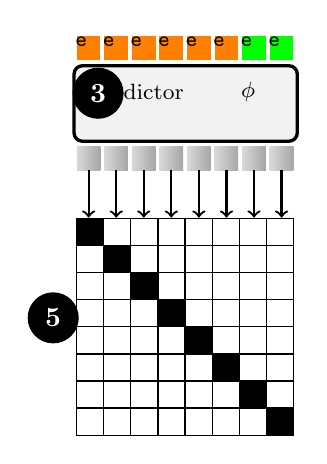
\begin{tikzpicture}
        
      \fill[gray!10, rounded corners=\cornerradius] (-0.01*\rectHeight, -0.138*\rectWidth) rectangle (0.8*\rectHeight, 0.501*\rectWidth);
      \draw[black, very thick, rounded corners=\cornerradius] (-0.01*\rectHeight, -0.138*\rectWidth) rectangle (0.8*\rectHeight, 0.501*\rectWidth);

      \def\COLORS_TARGET{{"orange", "orange", "orange", "orange", "orange", "orange", "green", "green"}}
      
      \foreach \i in {1,...,8} {    
        \pgfmathparse{\COLORS_TARGET[\i-1]} 
        \edef\THIS_COLOR{\pgfmathresult}
    
        % Draw the solid colored background square
        \fill[color=\THIS_COLOR] 
            (0.1*\i*\rectHeight - 0.1*\rectHeight, 0.5*\rectWidth + 0.25*\rectWidth)
            rectangle (0.1*\i*\rectHeight - 0.1*\rectHeight + 0.2*\rectWidth, 0.5*\rectWidth + 0.25*\rectWidth - 0.2*\rectWidth);
            
        \node[font=\footnotesize, align=center] at (0.1*\i*\rectHeight - 0.084*\rectHeight, 0.705*\rectWidth) {$\mathtt{e}$};
      }
      
      \foreach \i in {1,...,8} {
        \shade[shading=randomgray] (0.1*\i*\rectHeight - 0.1*\rectHeight, -0.384*\rectWidth) 
          rectangle (0.1*\i*\rectHeight - 0.1*\rectHeight + 0.2*\rectWidth, -0.184*\rectWidth); 
        \draw[->, thick] (0.1*\i*\rectHeight - 0.057*\rectHeight, -0.385*\rectWidth) -- (0.1*\i*\rectHeight - 0.057*\rectHeight, -0.785*\rectWidth);

      }
    \def\squareWidth{0.229}
    
    \foreach \row in {1,...,8} {
        \foreach \col in {1,...,8} {
            % Check if the current cell is on the diagonal
            \ifnum\row=\col
                % Fill the diagonal square with black
                \fill[black] 
                    (\squareWidth*\col*\rectWidth - \squareWidth*\rectWidth, -0.384*\rectWidth - \squareWidth*\row*\rectWidth - 0.41*\rectWidth) 
                    rectangle (\squareWidth*\col*\rectWidth, -0.384*\rectWidth - \squareWidth*\row*\rectWidth + \squareWidth*\rectWidth - 0.41*\rectWidth);
            \fi
            
            % Draw the black outline for each square
            \draw 
                (\squareWidth*\col*\rectWidth - \squareWidth*\rectWidth, -0.384*\rectWidth - \squareWidth*\row*\rectWidth - 0.41*\rectWidth) 
                rectangle (\squareWidth*\col*\rectWidth, -0.384*\rectWidth - \squareWidth*\row*\rectWidth + \squareWidth*\rectWidth - 0.41*\rectWidth);
            
        }
    }

      \node[font=\footnotesize, align=center] at (0.5*\rectWidth, 0.12*\rectHeight) {Predictor};
      \node[circle, draw=black, fill=black, text=white, font=\bfseries, minimum size=0.1cm, align=center] at (0.18*\rectWidth, 0.115*\rectHeight) {3};
      \node[circle, draw=black, fill=black, text=white, font=\bfseries, minimum size=0.1cm, align=center] at (-0.2*\rectWidth, -0.7*\rectHeight) {5};
      \node[font=\footnotesize, align=center] at (1.45*\rectWidth, 0.12*\rectHeight) {$\phi$};
    \end{tikzpicture}
  };
  
  % Predictor RIGHT
  \node[inner sep=0, anchor=north west] at (0.858*\rectHeight, 2.993*\rightRectSpacing) {
    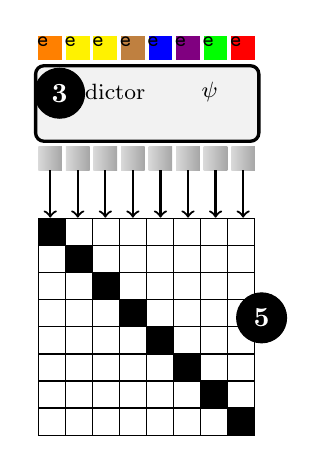
\begin{tikzpicture}
        
      \fill[gray!10, rounded corners=\cornerradius] (-0.01*\rectHeight, -0.138*\rectWidth) rectangle (0.8*\rectHeight, 0.501*\rectWidth);
      \draw[black, very thick, rounded corners=\cornerradius] (-0.01*\rectHeight, -0.138*\rectWidth) rectangle (0.8*\rectHeight, 0.501*\rectWidth);

      \def\COLORS_TARGET{{"orange", "yellow", "yellow", "brown", "blue", "violet", "green", "red"}}
      
      \foreach \i in {1,...,8} {    
        \pgfmathparse{\COLORS_TARGET[\i-1]} 
        \edef\THIS_COLOR{\pgfmathresult}
    
        % Draw the solid colored background square
        \fill[color=\THIS_COLOR] 
            (0.1*\i*\rectHeight - 0.1*\rectHeight, 0.5*\rectWidth + 0.25*\rectWidth)
            rectangle (0.1*\i*\rectHeight - 0.1*\rectHeight + 0.2*\rectWidth, 0.5*\rectWidth + 0.25*\rectWidth - 0.2*\rectWidth);
        \node[font=\footnotesize, align=center] at (0.1*\i*\rectHeight - 0.084*\rectHeight, 0.705*\rectWidth) {$\mathtt{e}$};
      }
      
      \foreach \i in {1,...,8} {
        \shade[shading=randomgray] (0.1*\i*\rectHeight - 0.1*\rectHeight, -0.384*\rectWidth) 
          rectangle (0.1*\i*\rectHeight - 0.1*\rectHeight + 0.2*\rectWidth, -0.184*\rectWidth); 
        \draw[->, thick] (0.1*\i*\rectHeight - 0.057*\rectHeight, -0.385*\rectWidth) -- (0.1*\i*\rectHeight - 0.057*\rectHeight, -0.785*\rectWidth);
      }
    \def\squareWidth{0.229}
    
    \foreach \row in {1,...,8} {
        \foreach \col in {1,...,8} {
            % Check if the current cell is on the diagonal
            \ifnum\row=\col
                % Fill the diagonal square with black
                \fill[black] 
                    (\squareWidth*\col*\rectWidth - \squareWidth*\rectWidth, -0.384*\rectWidth - \squareWidth*\row*\rectWidth - 0.41*\rectWidth) 
                    rectangle (\squareWidth*\col*\rectWidth, -0.384*\rectWidth - \squareWidth*\row*\rectWidth + \squareWidth*\rectWidth - 0.41*\rectWidth);
            \fi
            
            % Draw the black outline for each square
            \draw 
                (\squareWidth*\col*\rectWidth - \squareWidth*\rectWidth, -0.384*\rectWidth - \squareWidth*\row*\rectWidth - 0.41*\rectWidth) 
                rectangle (\squareWidth*\col*\rectWidth, -0.384*\rectWidth - \squareWidth*\row*\rectWidth + \squareWidth*\rectWidth - 0.41*\rectWidth);
            
        }
    }

      \node[font=\footnotesize, align=center] at (0.5*\rectWidth, 0.12*\rectHeight) {Predictor};
      \node[circle, draw=black, fill=black, text=white, font=\bfseries, minimum size=0.1cm, align=center] at (0.18*\rectWidth, 0.115*\rectHeight) {3};
      
      \node[circle, draw=black, fill=black, text=white, font=\bfseries, minimum size=0.1cm, align=center] at (1.89*\rectWidth, -0.7*\rectHeight) {5};
      \node[font=\footnotesize, align=center] at (1.45*\rectWidth, 0.12*\rectHeight) {$\psi$};
    \end{tikzpicture}
  };

\end{tikzpicture}